\subsection{Variables selection \label{variables_selection}}
\subsubsection{Correlations with the river discharge.\label{section231}}

Despite the variables' removal done in the \nameref{section212} section, we still have too many variables in our datasets.
Thus, we need to reduce this number and to focus only on the essential variables. So we perform an advanced statistical analysis.

First, we calculate the correlation matrix and we focus on the most correlated variables with the river discharge $Q$ (see Figure \ref{fig:corH} and Figure \ref{fig:corP}).
\begin{figure}[H]
\centering
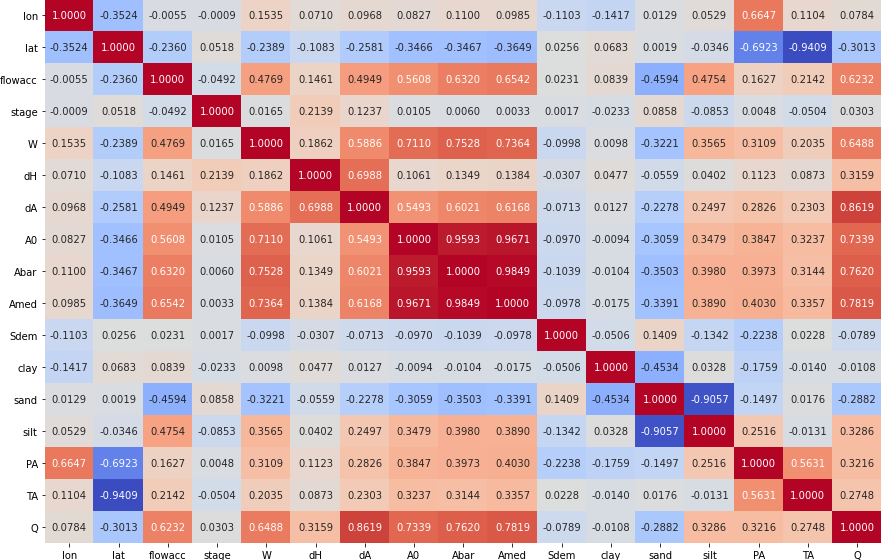
\includegraphics[scale=0.4]{Graph/correlation_hydro.png}
\caption{Correlation matrix of the HydroSwot dataset}
\label{fig:corH}
\end{figure}

For HydroSwot, we see in Figure \ref{fig:corH} that the highest coefficients of correlation with $Q$ are $dA$, $Abar$, $A0$, $Amed$, $W$, and $flowacc$. On the one hand, it makes sense to see $Abar$, $A0$, and $Amed$ so high because they are part of the equation to compute $Q$. On the other hand, $dA$, $W$, and $flowacc$ appear to be variables the most correlated with $Q$. In contrast, $Sdem$ is not highly correlated with $Q$.

\begin{figure}[H]
\centering
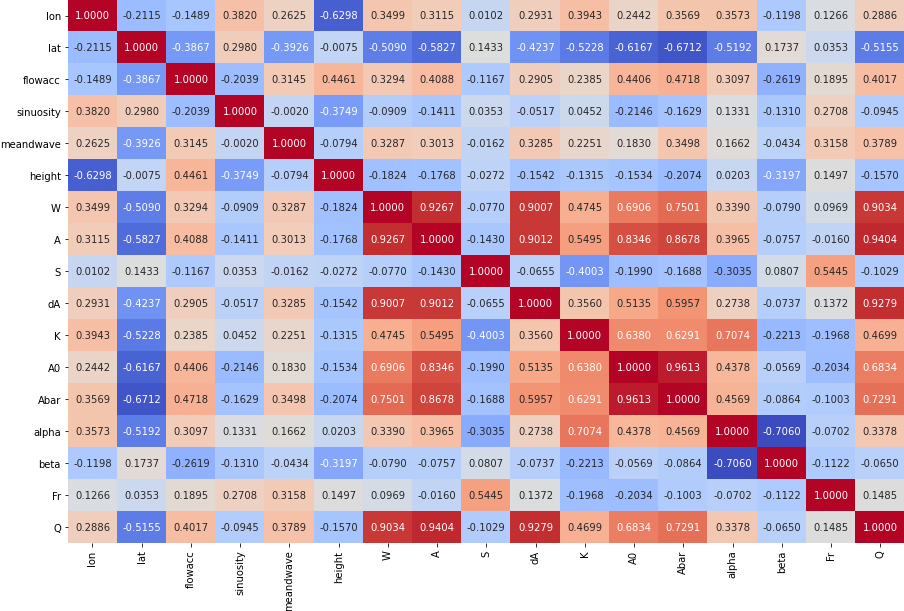
\includegraphics[scale=0.4]{Graph/correlation_pepsi.png}
\caption{Correlation matrix of the PEPSI dataset}
\label{fig:corP}
\end{figure}

For Pepsi, we calculate the correlations in figure \ref{fig:corP}. As for HydroSwot, we observe that $dA$ and $W$ are the two most correlated variables with the river discharge $Q$. But this time, $flowacc$ is much less correlated with $Q$, and the Strickler coefficient $K$ has a high coefficient correlation with $Q$.\newline

To conclude the analysis of the correlation coefficients, the most essential variables that explain $Q$ seem to be $dA$, $W$, and $flowacc$. We verify this conclusion with a Principal Component Analysis. 

\subsubsection{Principal Component Analysis.}

The first step of a PCA is to determine the number of principal components. Due to the high dimension of our datasets, the boxplot of the components is hardly sufficient to determine an optimal number of principal axes (see Figure \ref{fig:pcahydro} and Figure \ref{fig:pcapepsi}). 
 
 \begin{figure}[H]
     \centering
     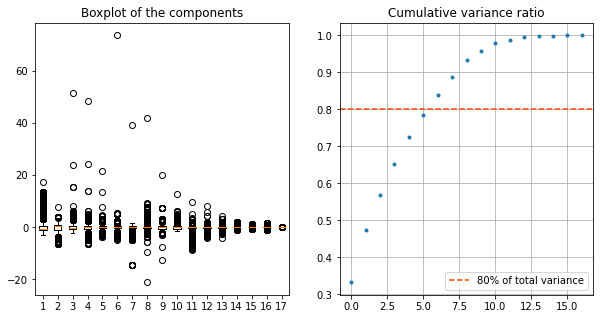
\includegraphics[scale = 0.55]{Graph/hydro_pca.png}
     \caption{Boxplot of the components and cumulative variance ratio plot, HydroSwot dataset}
     \label{fig:pcahydro}
 \end{figure}
 
Although we cannot determine the exact number of components using the boxplot, the plot of the cumulative variance ratio (see Figure \ref{fig:pcahydro}) shows that 6 components are sufficient to almost reach $80\%$ of the total variance for the HydroSwot dataset.

 \begin{figure}[H]
     \centering
     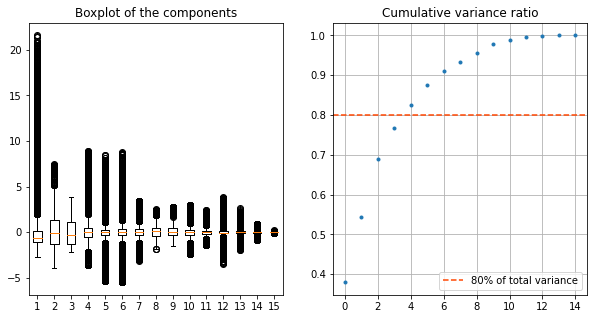
\includegraphics[scale = 0.55]{Graph/pepsi_pca.png}
     \caption{Boxplot of the components and cumulative variance ratio plot, PEPSI dataset}
     \label{fig:pcapepsi}
 \end{figure}

For the PEPSI dataset, 4 components seem to be sufficient. Taking a fifth principal component to reach $80\%$ of the total variance just represents a small ratio of variance, so we decide to take 4 principal axes.

Then, we show the loading plots. We want to find the major interactions, so we focus on the spans formed by the two first principal components (See Figure \ref{fig:factormap}).

\begin{figure}[H]
    \centering
    \begin{subfigure}{0.45\textwidth}
        \centering
        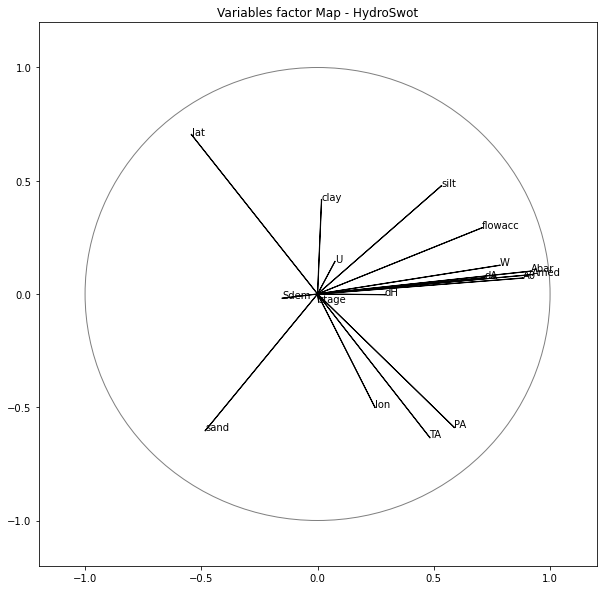
\includegraphics[scale=0.28]{Graph/factor_map_hydro.png}
        \caption{HydroSwot}
        \label{subfig:fmh}
    \end{subfigure}
    \begin{subfigure}{0.45\textwidth}
        \centering
        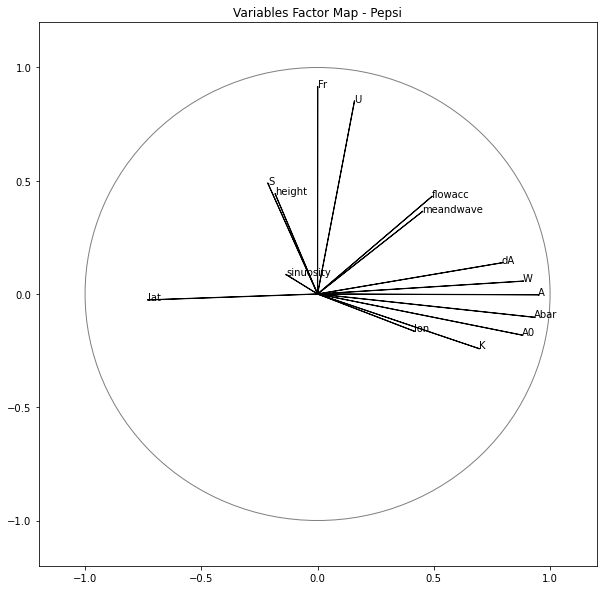
\includegraphics[scale=0.28]{Graph/factor_map_pepsi.png}
        \caption{PEPSI}
        \label{subfig:fmp}
    \end{subfigure}
\caption{Loading plots in the span formed by components 1 and 2}
\label{fig:factormap}
\end{figure}

As we can see on Figure \ref{subfig:fmh}, for HydroSwot, the variables that most explain the principal component are $dA$, $W$, and $flowacc$, as the first two ones are almost parallel to the first axe. We also notice the importance of the composition of the river with $sand$ and $silt$, the meteorological data with $PA$ and $TA$, and finally the geographical position. 

As for HydroSwot, $dA$, $W$, and $flowacc$ are good descriptors of the first component of the PEPSI dataset (see Figure \ref{subfig:fmp}). This time, we observe that the slope $S$ is part of the significant variables. Once again, we observe the importance of the physical metric such as the Froude Number, $Fr$, and the Strickler coefficient, $K$.\newline

Finally, we display the score plots in the span formed by the two principal components (see Figure \ref{fig:scoreplot}).

\begin{figure}[H]
    \centering
    \begin{subfigure}{0.45\textwidth}
        \centering
        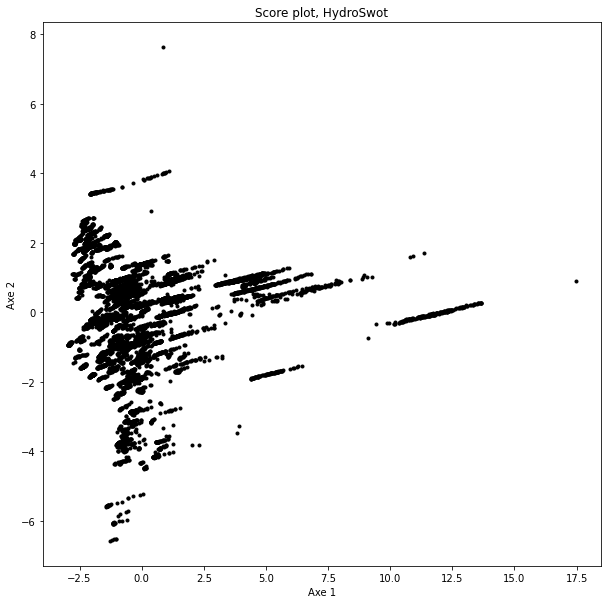
\includegraphics[scale=0.28]{Graph/scoreplot_hydro.png}
        \caption{HydroSwot}
        \label{subfig:sph}
    \end{subfigure}
    \begin{subfigure}{0.45\textwidth}
        \centering
        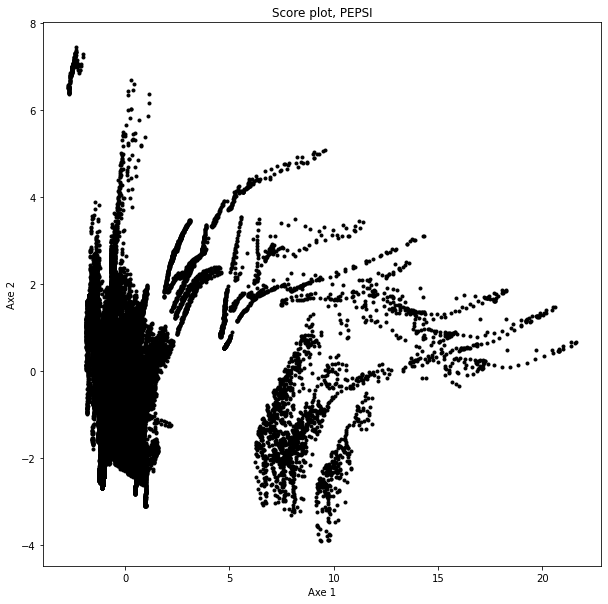
\includegraphics[scale=0.28]{Graph/scoreplot_pepsi.png}
        \caption{PEPSI}
        \label{subfig:spp}
    \end{subfigure}
\caption{Score plots in the span formed by components 1 and 2}
\label{fig:scoreplot}
\end{figure}

Concerning the HydroSwot dataset, we observe in Figure \ref{subfig:sph} that the individuals form lines whose directions are similar to the directions of $dA$, $W$, and $flowacc$ on the loading plot of HydroSwot (see Figure \ref{subfig:fmh}). It stresses the fact that these variables are very significant (see \nameref{section231} section) in this dataset, and it suggests that each line represents all the observations of a particular river.

We see in Figure \ref{subfig:spp} that the individuals from the PEPSI dataset have a singular representation, but it is difficult to analyse the meaning of it. Even so, we notice two different groups, that may correspond to two different scale of river discharge.\newline

To  summarise, the multidimensional analysis leads us to use four input variables for the neural networks : $W$, $dA$, $flowacc$, and the slope ($Sdem$ for HydroSwot, and $S$ for Pepsi, which seems to be more significant than $Sdem$).

\subsubsection{River Classification.\label{section233}} 

To have the most accurate flow estimation, we split rivers into groups. We need to define the number of groups and how to determine them.

We compute a K-means classification for the two datasets with 2 and 3 groups. More groups would lead to too small groups, i.e. with not enough observations to run neural networks algorithms. For both datasets, the K-means classification on 2 groups determines a huge group with the majority of the observations and the other with the rest of the observations. The K-means classification with 3 groups leads to 2 equivalent groups in size and the third group remains small.  

Figure \ref{fig:kmeans} shows a representation of classes by K-means for the HydroSwot dataset. We notice that K-means separates groups distinctly. It also suggests that observations from the same river can be in several groups. K-means classification does not separate rivers between them, it suggests to separate data by river portions.

\begin{figure}[H]
    \begin{subfigure}{0.45 \textwidth}
        \centering
        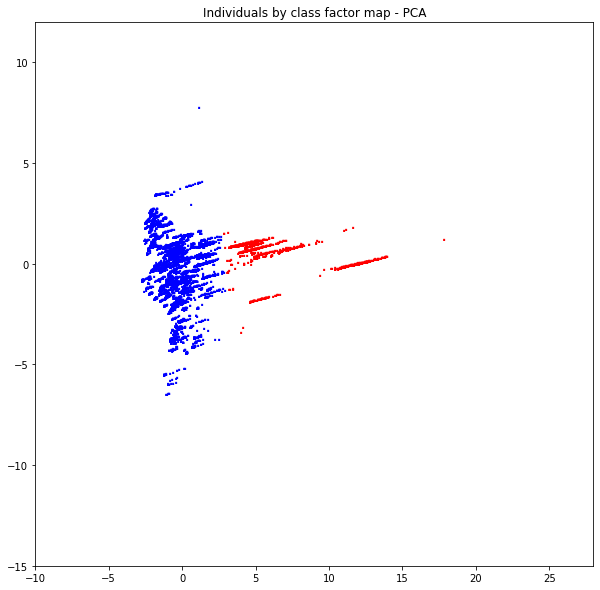
\includegraphics[scale = 0.3]{Graph/kmeans2HS.png}
        \caption{2 classes}
    \end{subfigure}
\centering
    \begin{subfigure} {0.45 \textwidth}
        \centering
        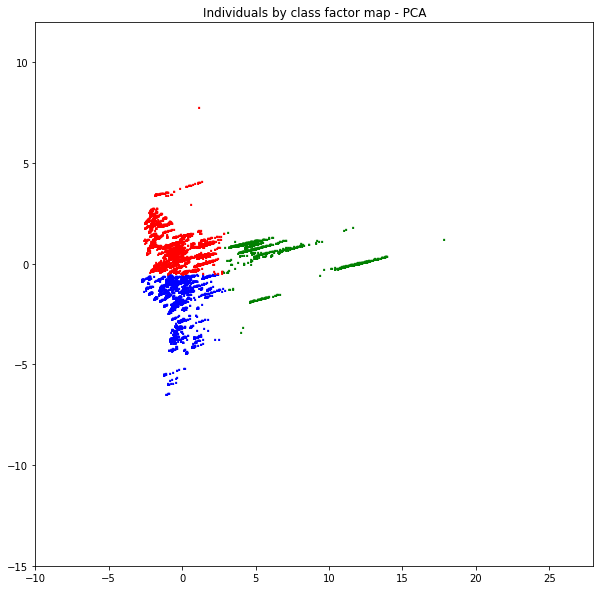
\includegraphics[scale = 0.3]{Graph/kmeans3HS.png}
        \caption{3 classes}
    \end{subfigure}
\caption{Plots for different numbers of classes in the span of the 2 first ACP components for Hydroswot }
\label{fig:kmeans}
\end{figure}

Splitting into 3 groups is not needed for our study. Indeed, we aim to have the largest dataset possible. 

We examine in figure \ref{fig:boxplot_hydro} boxplots of the different variables depending on groups determined by K-means for both datasets. We note that variables which distinct the 2 groups are mainly $Q$ and $flowacc$. $dA$ is also a good separator. \newline

\begin{figure}[H]
\begin{subfigure}{0.45\textwidth }
     \centering
        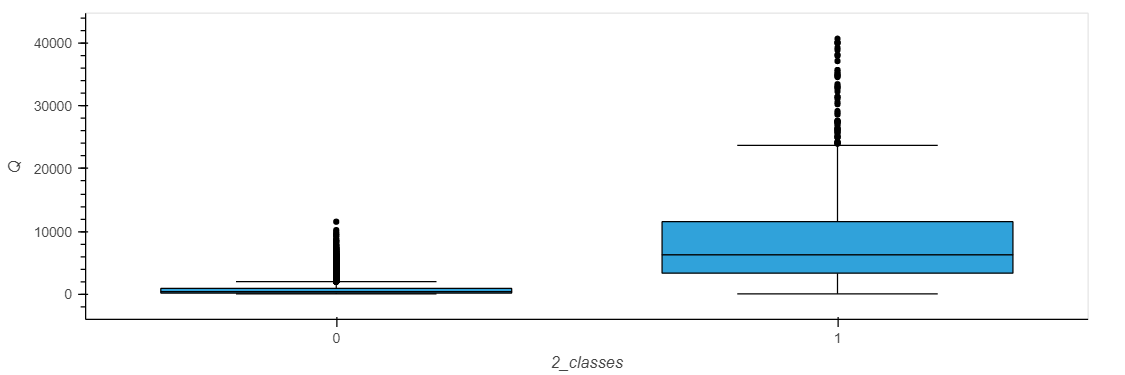
\includegraphics[scale = 0.19]{Graph/bokeh_plot.png}
        \caption{Boxplot of Q}
\end{subfigure}
\begin{subfigure}{0.45\textwidth}
     \centering
        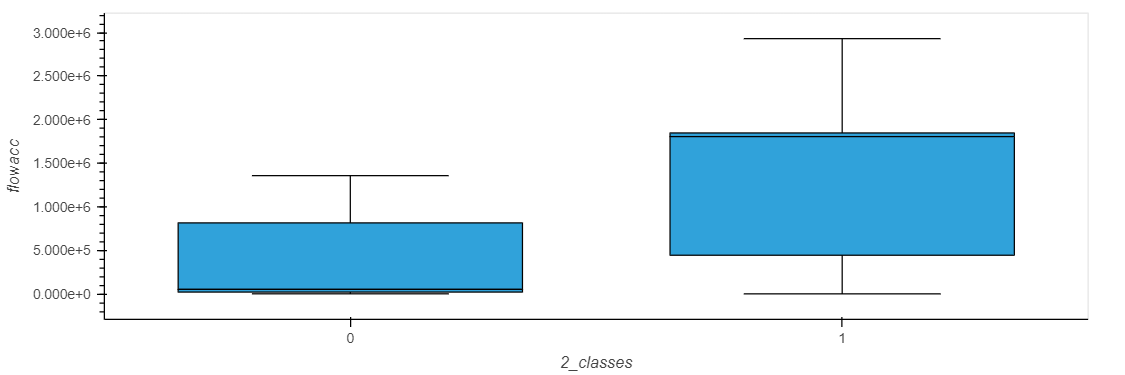
\includegraphics[scale = 0.19]{Graph/flowacc_hydro.png}
        \caption{Boxplot of flowacc }
\end{subfigure}
  \caption{Boxplots of different variables for 2 HydroSwot classes}     
  \label{fig:boxplot_hydro}
\end{figure}

\underline{Remark:} we do not show results of K-means classification for the PEPSI dataset because we obtain the same results and conclusions. \\
    
We finally choose two ways to separate rivers for both datasets. Each method separate rivers into 2 groups as we do not have enough data to create 3 groups.

First, we group data by rivers and compute the river flow mean. We separate them using the criteria of $Q$ which is a good separator according to K-means method. For HydroSwot, we make 2 groups: high discharge rivers ($Q > 1000 m^3/s$) and low discharge rivers ($Q < 1000 m^3/s$). For Pepsi we fix the boundary at $3000 m^3/s$. We notice that the high discharge rivers group for PEPSI contains only 3 rivers: $Mississipi$, $Padma$ and $Jamuna$. This separation by entire rivers is close to the real context of the SWOT Mission. For LSTM network, we will train and test on entire rivers that we know exactly. Then, we will use this algorithm on unknown rivers that the satellite would have measured. We name these separations Hydroswot/PEPSI Handmade - Low/High $Q$.\\

\underline{Remark :} we could separate the datasets using $flowacc$ as we saw that it is also a good separator. \\
The second way to separate data is by following K-means method to split Hydroswot and Pepsi into 2 classes. Among separative variables we have $Q$, so we decide to name the two classes with Low $Q$ and High $Q$. Thus, we obtain Table \ref{Tab:class_prop}.

\begin{table}[H]
\centering
    \begin{tabular}{|c|c|c|}
    \hline
    & Low $Q$ & High $Q$ \\ \hline
    Hydroswot Handmade & 6714 & 5129 \\\hline
    Pepsi Handmade & 47548 & 3721 \\\hline
    Hydroswot K-means  &  10490 & 1140 \\\hline
    Pepsi K-means & 47536 & 2674\\ \hline
    \end{tabular}
\caption{Number of observations in the different classes}
\label{Tab:class_prop}
\end{table}

We notice that HydroSwot K-means - High $Q$ has only 1140 observations. This small number may impact the efficiency of neural networks.